

\documentclass{beamer}
\usepackage[utf8]{inputenc}
\usepackage[frenchb]{babel}
\usepackage[T1]{fontenc}
\usetheme{Darmstadt}
\usecolortheme{beaver}


\usepackage{pgfplots}

\usepackage{graphicx}


\title{Sparse Representation}
\author{Nicolas Lupinski \& Gregory Potdevin \& Rémy El Sibaïe Besognet}

\definecolor{light-gray}{gray}{0.80}

\begin{document}

\begin{frame}
  \titlepage  
\end{frame}


\begin{frame}{Introduction}

\begin{block}{Previous optimizations}
\begin{itemize}
\item 64 bits hash
\item small cardinalities : linear counting
\item no bias ($n < 65000$)
\end{itemize}
\end{block}


\begin{block}{Goals}
\begin{itemize}
\item Accuracy
\item Memory efficiency
\item \only<1>{Estimate large cardinalities} \only<2->{\textcolor{light-gray}{Estimate large cardinalities}}
\item \only<1>{Practicality} \only<2->{\textcolor{light-gray}{Practicality}}
\end{itemize}
\end{block}


\end{frame}

%% ============================


\begin{frame}{Why use a sparse representation}


\begin{block}{HyperLogLog}
Fixed amount of memory depending on the precision ($6\times m$ bits)

($\varrho(w)$ : 6 bits)
\end{block}

\begin{figure}[c]
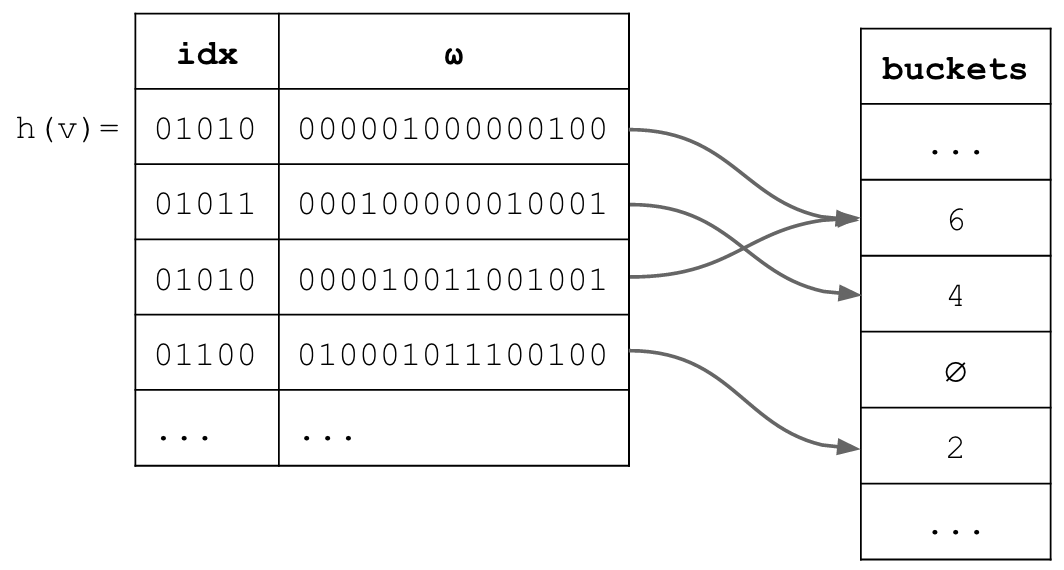
\includegraphics [scale=0.4]  {hyperloglog_buckets.png}
\end{figure}


\begin{block}{Memory efficieny}
Should use less memory for low cardinalities
\begin{itemize}
\item when $n \ll m$, most of registers are never used 
\end{itemize}
\end{block}

\end{frame}

%% ============================

\begin{frame}{What sparse representation}


\begin{minipage}{0.5\textwidth}%
\begin{block}{Key/Value pairs}
\begin{itemize}
\item index as key
\item $\varrho(w)$ as value
\end{itemize}
\end{block}
\end{minipage}%
\hfill%
\begin{minipage}{0.5\textwidth}%
\begin{figure}[c]
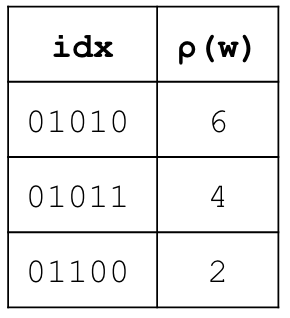
\includegraphics [scale=0.5]  {hyperloglog_list.png}
\end{figure}
\end{minipage}%


\begin{block}{Sparse representation}
\begin{itemize}
\item Stored as a integers (MSB for the index, LSB for the value)
\item Sorted list for faster lookups
\item Convert to the dense representation when the list grows too much : $6\times m < k\times (p + 6)$
\end{itemize}
\end{block}

\end{frame}


\begin{frame}{What sparse representation}


\begin{block}{Optimization : bufferize insertions}
\begin{itemize}
\item Compact sorted list of key/value integers
\item Speed up insertions with a set of values to insert
\item When the set reaches a maximum size
\begin{itemize}
\item Sort the set
\item Merge with the sorted list (linear time)
\end{itemize}
\end{itemize}
\end{block}

\end{frame}

%% ============================


\begin{frame}{Higher precision}


\begin{block}{Motivation}
\begin{itemize}
\item HyperLogLog is less efficient for low cardinalities. 
\item Sparse representation for low cardinalities... optimize for this use case !
\end{itemize}
\end{block}

Higher precision is obtained by using more bits for the index. 

\begin{block}{Note}
\begin{itemize} 
\item At most 6 bits are used for $\varrho(w)$
\item Remaining bits can be used for the index
\item If all bits are used for the index... we have Linear Counting
\end{itemize}
\end{block}

\end{frame}



\begin{frame}{Higher precision}


\begin{block}{Convert to dense representation}
Sparse representation uses p' bits for the index, with $p' \ge p$

TODO !
\end{block}

\end{frame}

\begin{frame}{Higher precision}


\begin{figure}[c]
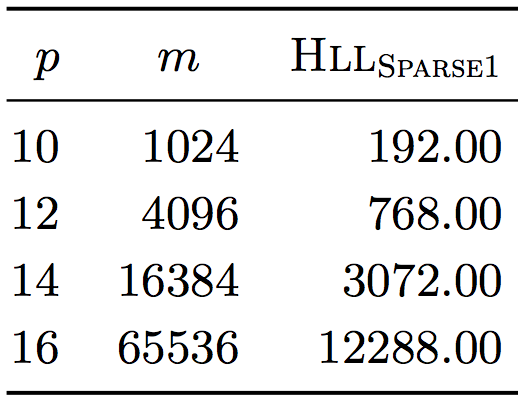
\includegraphics [scale=0.45]  {sparse1.png}

Maximum key/value number ($p' = 25$)
\end{figure}

\end{frame}

%% ============================


\begin{frame}{Compressed sparse representation}


\begin{block}{Motivation}
\begin{itemize}
\item Memory efficiency for low cardinalities
\item Use knowledge we have of the data structures
\end{itemize}
\end{block}


\begin{block}{Data structures}
\begin{itemize}
\item Set buffer
  \begin{itemize}
  \item compact integers, low memory footprint
  \end{itemize}
\item Sorted list
  \begin{itemize}
  \item Variable length encoding
  \item Difference encoding
  \end{itemize}
\end{itemize}
\end{block}


\end{frame}



\begin{frame}{Difference encoding}

\begin{figure}[c]
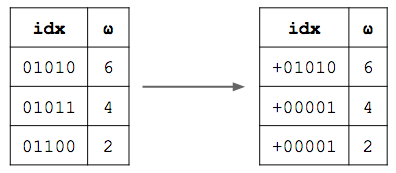
\includegraphics [scale=0.5]  {hyperloglog_difference.png}
\end{figure}


\end{frame}

\begin{frame}{Compressed sparse representation}


\begin{figure}[c]
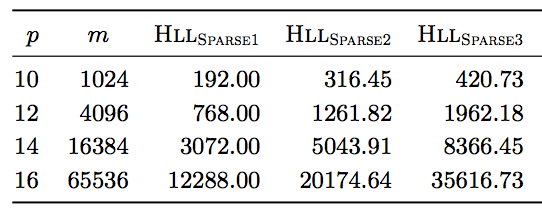
\includegraphics [scale=0.45]  {sparse123.png}

Maximum key/value number ($p' = 25$)
\end{figure}

\end{frame}

%% ============================
\begin{frame}{Encoding hash values}

  We need a bigger encoding if we switch to the normal representation
  and if $\langle x_{63}, \dots, x_{64-p\prime} \rangle$ are all 0.
  ~\\
  \colorbox{light-gray}{$\langle x_{63}, \dots, x_{64-p\prime} \rangle \| \langle \varrho (w\prime) \rangle \| \langle 1 \rangle $}

  ~\\
  In the other cases:
  \colorbox{light-gray}{$\langle x_{63}, \dots, x_{64-p\prime} \rangle \| \langle 0 \rangle $}

  ~\\
  The gain of space on the hashed values increases precision ($p\prime)$

\end{frame}


%% ============================

\begin{frame}{Space efficieny}
  
\begin{figure}[c]
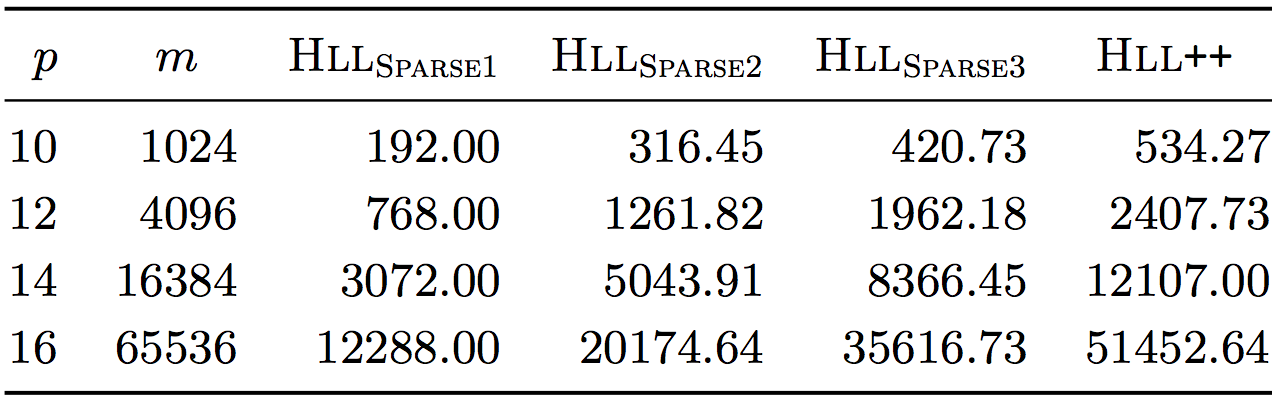
\includegraphics [scale=0.45]  {sparse_all.png}

Maximum key/value number ($p' = 25$)
\end{figure}
\end{frame}



\begin{frame}{Conclusion : Median relative error}
\begin{figure}[c]
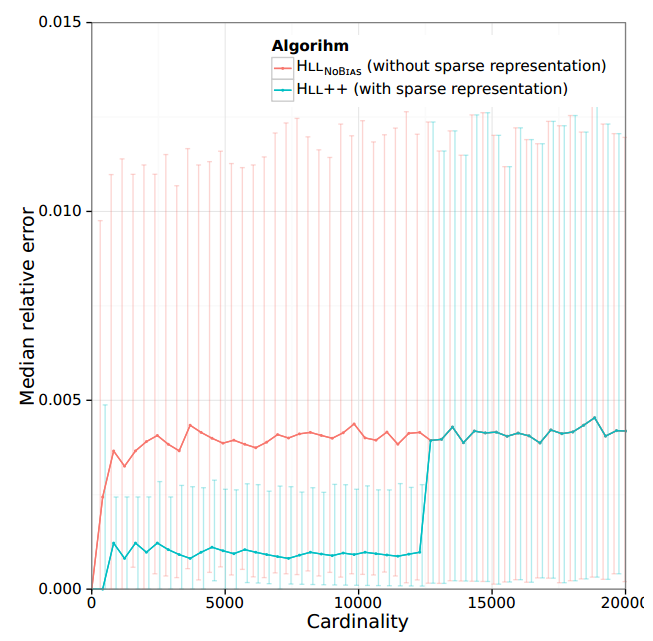
\includegraphics [scale=0.30]  {hll_fig5.png}

HLLnobias vs HLL++
\end{figure}
\end{frame}


\begin{frame}{Conclusion}

\begin{block}{Optimisations}
\begin{itemize}
\item Higher precision
\item Compression
\item Encoding hash values
\end{itemize}
\end{block}


\begin{block}{Benefits}
\begin{itemize}
\item Smaller memory footprint
\item Increased accuracy
\item Larger high precision range 
\end{itemize}
\end{block}

\end{frame}





\end{document}



(*
% rubber: setlist arguments --shell-escape --enable-write18
Local Variables:
compile-command: "rubber -d slides.tex"
ispell-local-dictionary: "francais"
End:
*)



